\documentclass[12pt]{article}

\usepackage{amssymb,amsmath,amsfonts,eurosym,geometry,ulem,graphicx,caption,color,setspace,sectsty,comment,footmisc,caption,natbib,pdflscape,subfigure,array,hyperref,booktabs}

\geometry{left=1.0in,right=1.0in,top=1.0in,bottom=1.0in}

\makeatletter
\setlength{\@fptop}{0pt}
\makeatother

\begin{document}

\title{Comparative statics}
\maketitle

\section{Comparative statics on $\theta_S$}

\subsection{Exercise 1}

\begin{table}[htbp]
	\centering
	\caption{Parameters exercise 1}
	\begin{tabular}{lr}
		\toprule
		Parameter & \multicolumn{1}{l}{Value} \\
		\midrule
		&  \\
		Periods per year & 1.000 \\
		$\beta$ & 0.960 \\
		Life expectancy & 45.000 \\
		$\delta$ & 0.022 \\
		$A$ & 0.500 \\
		$\alpha$ & 0.500 \\
		$\kappa$ & 0.200 \\
		$\bar {c}$ & 0.500 \\
		$\lambda$ & 0.500 \\
		$\gamma$ & 1.500 \\
		&  \\
		Gender wage gap & 0.750 \\
		Skill premium & 0.250 \\
		General wage level & 1.000 \\
		\bottomrule
	\end{tabular}
\end{table}


\begin{figure}
	\centering
	\caption{Value of being single}
	\subfigure[Females]{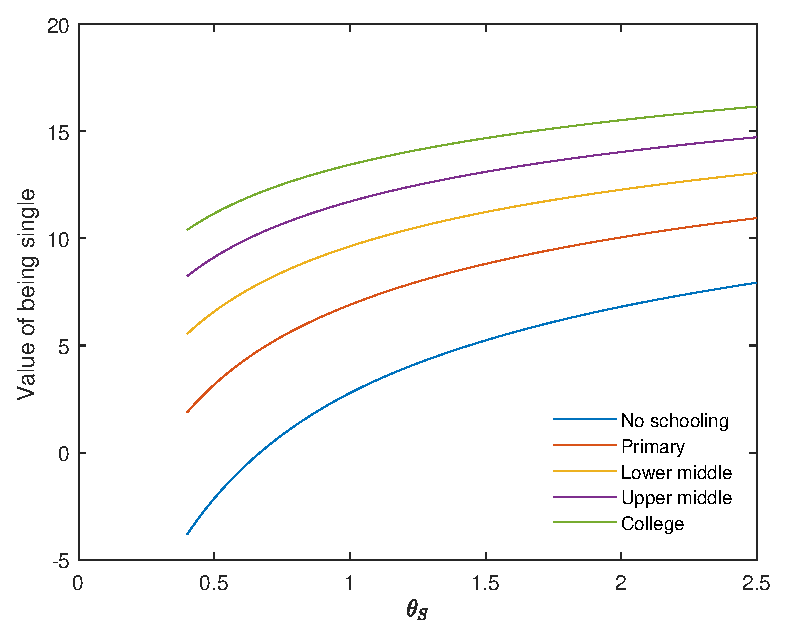
\includegraphics{Graphs/VS_f_theta_S_ex1.eps}} \\
	\subfigure[Males]{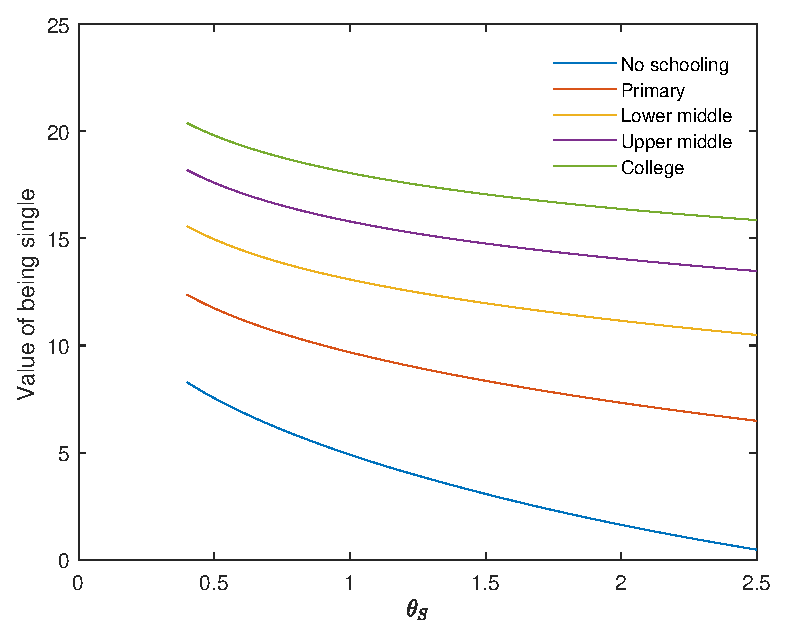
\includegraphics{Graphs/VS_m_theta_S_ex1.eps}}
\end{figure}


\begin{figure}
	\centering
	\caption{Matching probability by sex}
	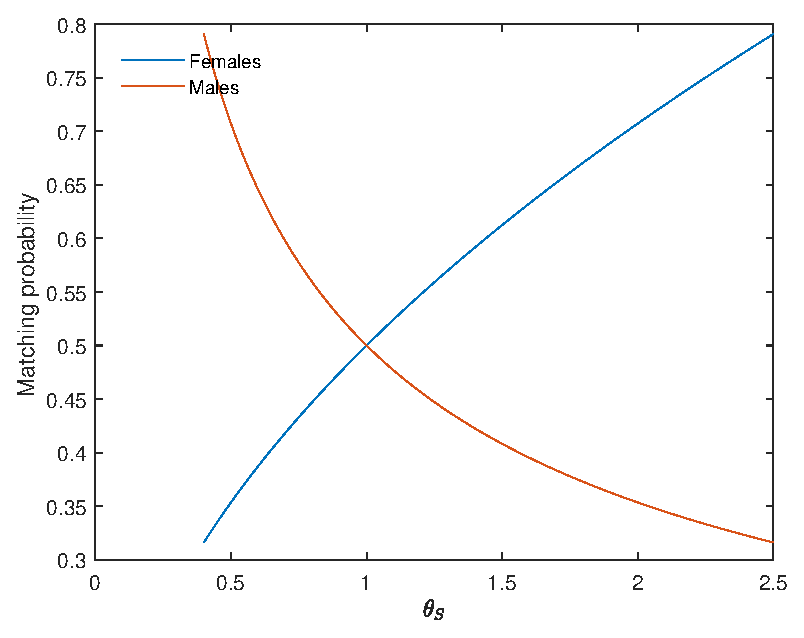
\includegraphics{Graphs/match_prob_theta_S_ex1.eps}
\end{figure}

\begin{figure}
	\centering
	\caption{Marriage rates by sex}
	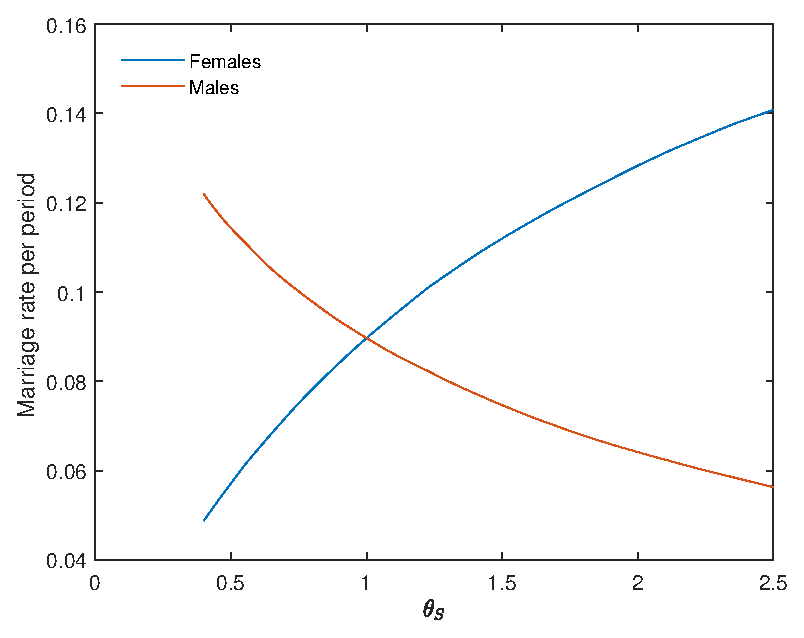
\includegraphics{Graphs/marr_rates_theta_S_ex1.eps}
\end{figure}

\begin{figure}
	\centering
	\caption{Marriage rates by education level}
	\subfigure[Females]{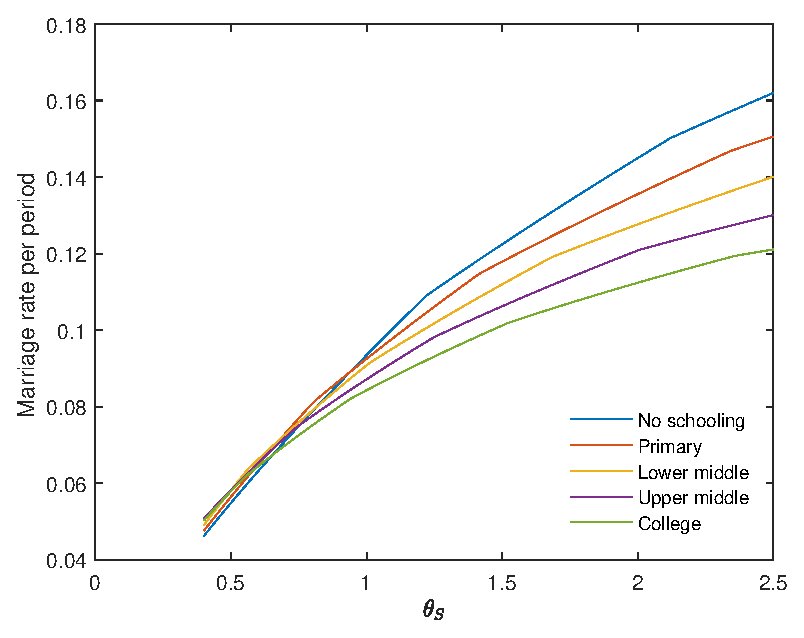
\includegraphics{Graphs/MR_f_theta_S_ex1.eps}} \\
	\subfigure[Males]{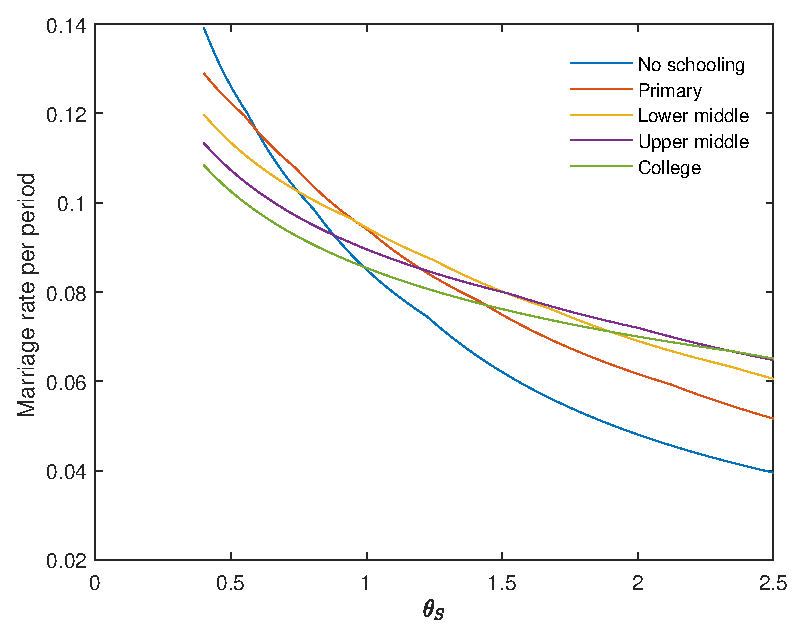
\includegraphics{Graphs/MR_m_theta_S_ex1.eps}}
\end{figure}

\begin{figure}
	\centering
	\caption{Marital sorting in education}
	\subfigure[Basis: only married people]{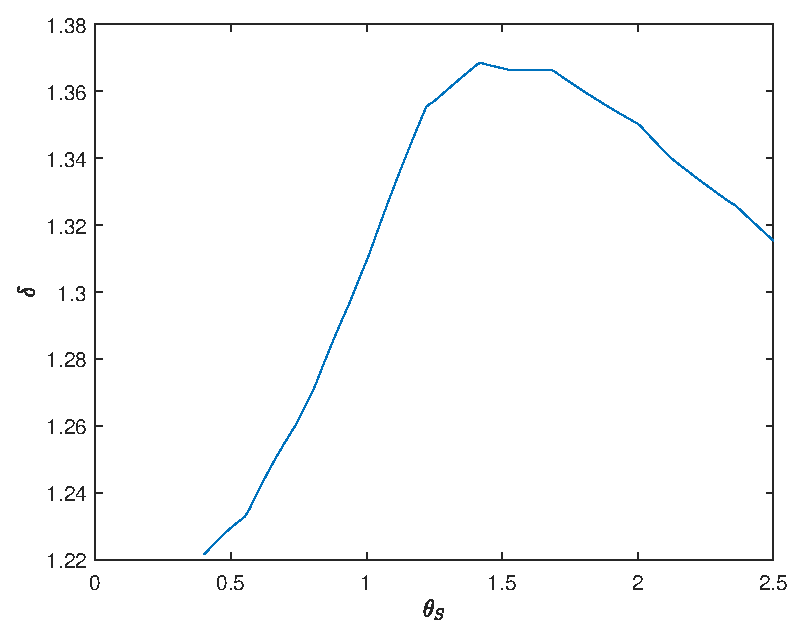
\includegraphics{Graphs/sorting_theta_S_ex1.eps}} \\
	\subfigure[Basis: all individuals]{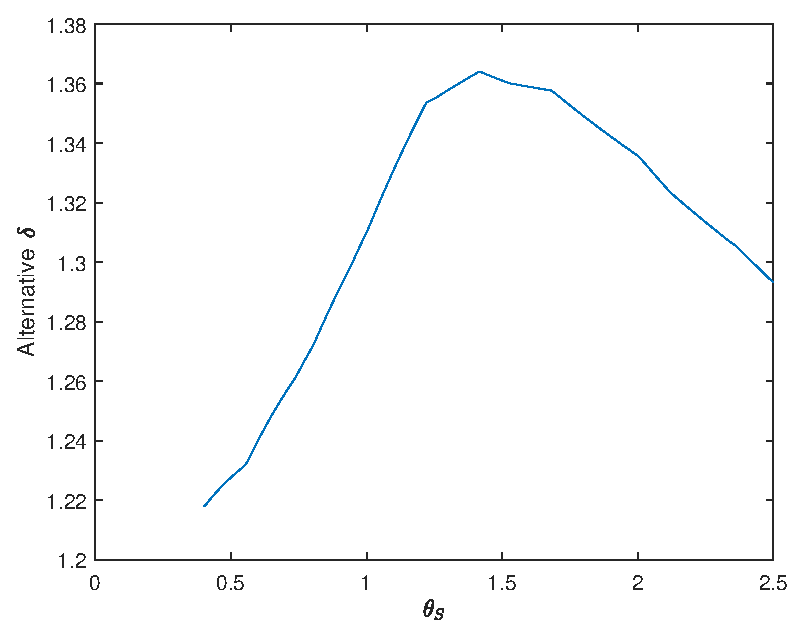
\includegraphics{Graphs/sorting_2_theta_S_ex1.eps}}
\end{figure}

\begin{figure}
	\centering
	\caption{Hypergamy in education by sex}
	\subfigure[Basis: only married people]{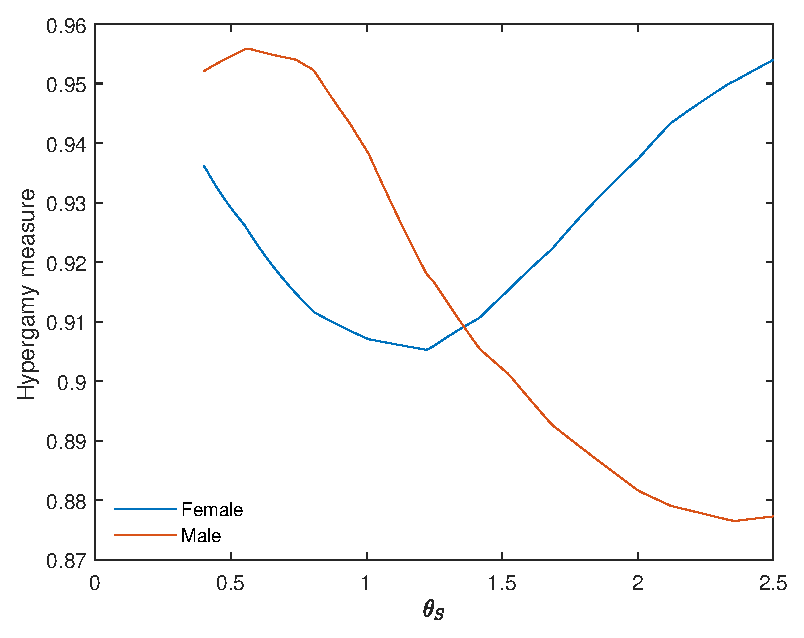
\includegraphics{Graphs/hypergamy_theta_S_ex1.eps}} \\
	\subfigure[Basis: all individuals]{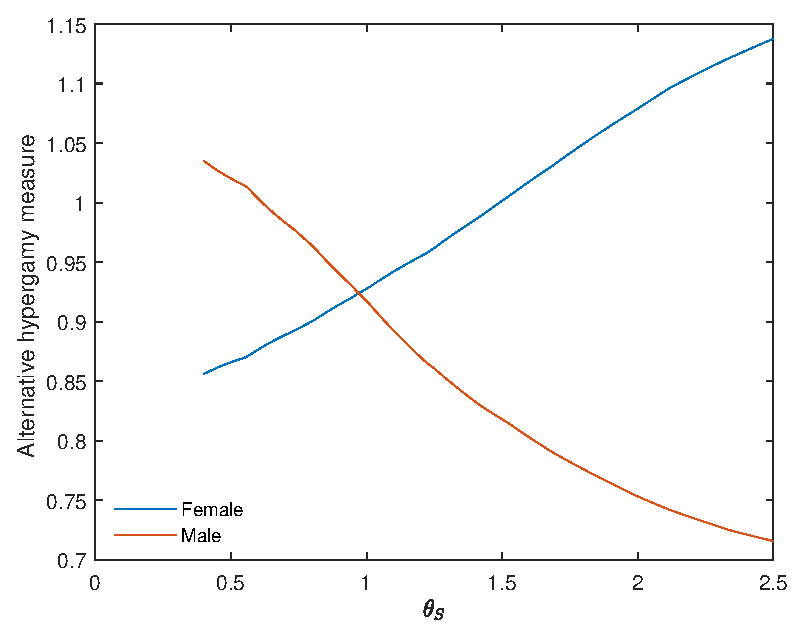
\includegraphics{Graphs/hypergamy_2_theta_S_ex1.eps}}
\end{figure}


\begin{figure}
	\centering
	\caption{Expected time to marriage}
	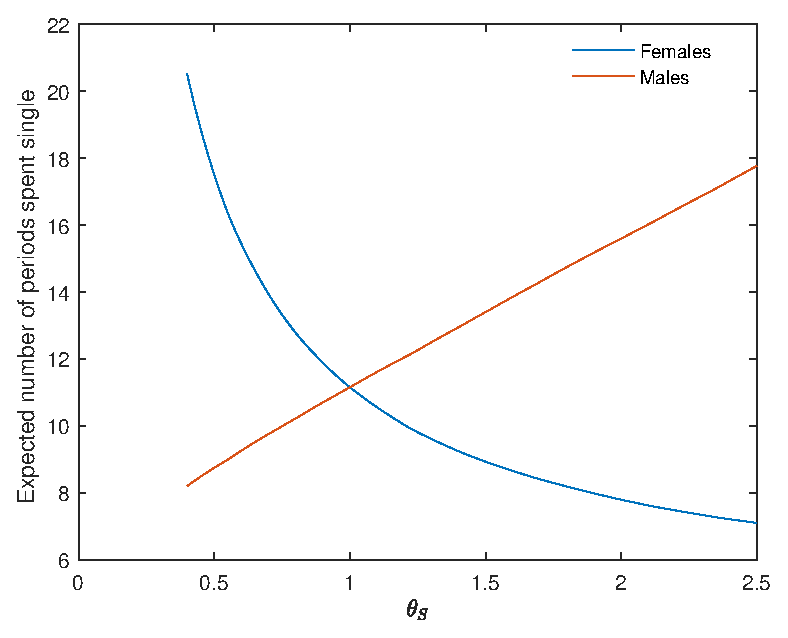
\includegraphics{Graphs/exp_single_theta_S_ex1.eps}
\end{figure}

\begin{figure}
	\centering
	\caption{Married female labor supply}
	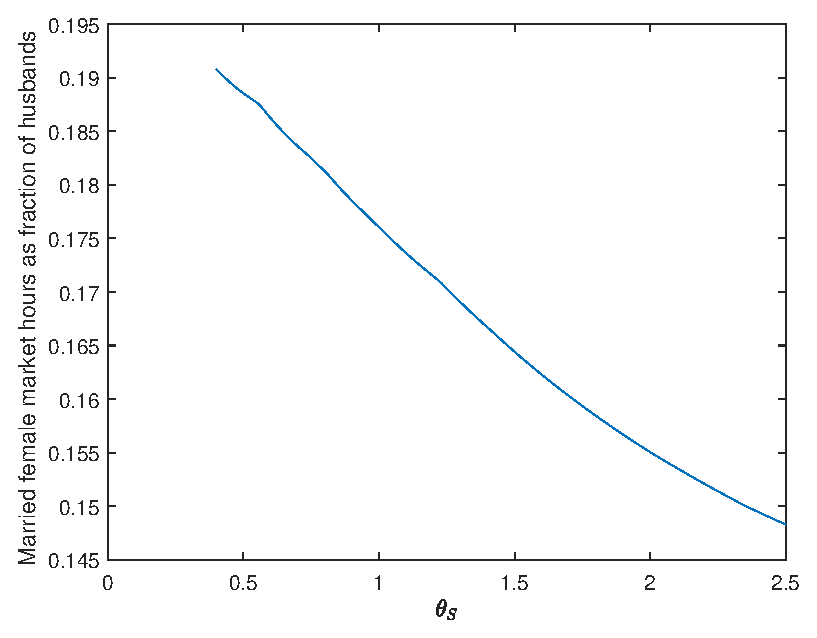
\includegraphics{Graphs/lf_theta_S_ex1.eps}
\end{figure}

\begin{figure}
	\centering
	\caption{Inequality}
	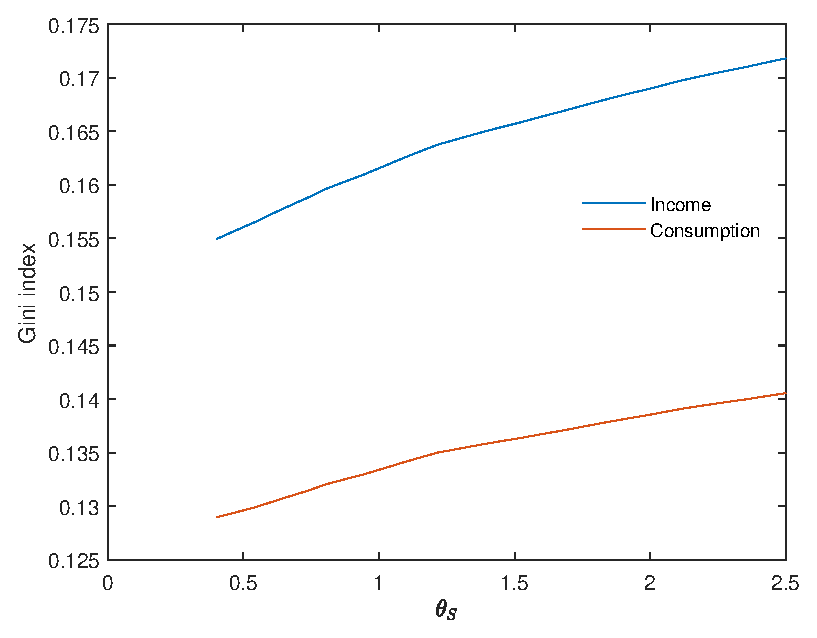
\includegraphics{Graphs/ineq_theta_S_ex1.eps}
\end{figure}

Notes:

\begin{enumerate}
	\item 
\end{enumerate}

\clearpage

\section{Comparative statics on the skill premium}

\subsection{Exercise 1}

\begin{table}[htbp]
	\centering
	\caption{Parameters for exercise 1}
	\begin{tabular}{lr}
		\toprule
		Parameter & \multicolumn{1}{l}{Value} \\
		\midrule
		&  \\
		Periods per year & 1,000 \\
		$\beta$ & 0,960 \\
		Life expectancy & 45,000 \\
		$\delta$ & 0,022 \\
		$A$ & 0,500 \\
		$\alpha$ & 0,500 \\
		$\kappa$ & 0,200 \\
		$\bar {c}$ & 0,500 \\
		$\lambda$ & 0,500 \\
		$\gamma$ & 1,500 \\
		&  \\
		$\theta_S$ & 1,500 \\
		&  \\
		Gender wage gap & 0,750 \\
		General wage level & 1,000 \\
		\bottomrule
	\end{tabular}
\end{table}

\begin{figure}
	\centering
	\caption{Value of being single}
	\subfigure[Females]{\includegraphics{Graphs/VS_f_skill_premium_ex1.eps}} \\
	\subfigure[Males]{\includegraphics{Graphs/VS_m_skill_premium_ex1.eps}}
\end{figure}


\begin{figure}
	\centering
	\caption{Matching probability by sex}
	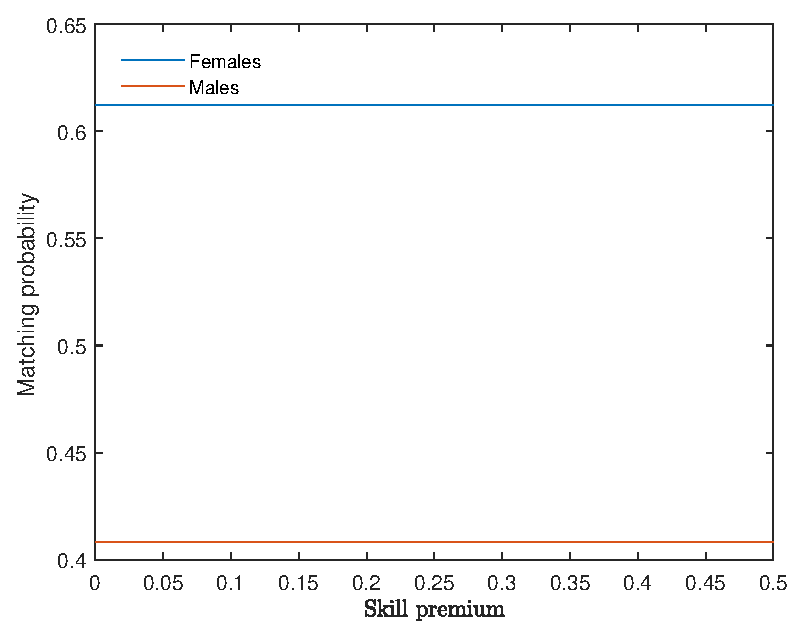
\includegraphics{Graphs/match_prob_skill_premium_ex1.eps}
\end{figure}

\begin{figure}
	\centering
	\caption{Marriage rates by sex}
	\includegraphics{Graphs/marr_rates_skill_premium_ex1.eps}
\end{figure}

\begin{figure}
	\centering
	\caption{Marriage rates by education level}
	\subfigure[Females]{\includegraphics{Graphs/MR_f_skill_premium_ex1.eps}} \\
	\subfigure[Males]{\includegraphics{Graphs/MR_m_skill_premium_ex1.eps}}
\end{figure}

\begin{figure}
	\centering
	\caption{Marital sorting in education}
	\subfigure[Basis: only married people]{\includegraphics{Graphs/sorting_skill_premium_ex1.eps}} \\
	\subfigure[Basis: all individuals]{\includegraphics{Graphs/sorting_2_skill_premium_ex1.eps}}
\end{figure}

\begin{figure}
	\centering
	\caption{Hypergamy in education by sex}
	\subfigure[Basis: only married people]{\includegraphics{Graphs/hypergamy_skill_premium_ex1.eps}} \\
	\subfigure[Basis: all individuals]{\includegraphics{Graphs/hypergamy_2_skill_premium_ex1.eps}}
\end{figure}


\begin{figure}
	\centering
	\caption{Expected time to marriage}
	\includegraphics{Graphs/exp_single_skill_premium_ex1.eps}
\end{figure}

\begin{figure}
	\centering
	\caption{Married female labor supply}
	\includegraphics{Graphs/lf_skill_premium_ex1.eps}
\end{figure}

\begin{figure}
	\centering
	\caption{Inequality}
	\includegraphics{Graphs/ineq_skill_premium_ex1.eps}
\end{figure}

Notes:

\begin{enumerate}
	\item 
\end{enumerate}

\clearpage

\section{Comparative statics on $A$}

\subsection{Exercise 1}

\begin{table}[htbp]
	\centering
	\caption{Parameters for exercise 1}
	\begin{tabular}{lr}
		\toprule
		Parameter & \multicolumn{1}{l}{Value} \\
		\midrule
		&  \\
		Periods per year & 1,000 \\
		$\beta$ & 0,960 \\
		Life expectancy & 45,000 \\
		$\delta$ & 0,022 \\
		$\alpha$ & 0,500 \\
		$\kappa$ & 0,200 \\
		$\bar {c}$ & 0,500 \\
		$\lambda$ & 0,500 \\
		$\gamma$ & 1,500 \\
		&  \\
		$\theta_S$ & 1,500 \\
		&  \\
		Gender wage gap & 0,750 \\
		Skill premium & 0,250 \\
		General wage level & 1,000 \\
		\bottomrule
	\end{tabular}
\end{table}

\begin{figure}
	\centering
	\caption{Value of being single}
	\subfigure[Females]{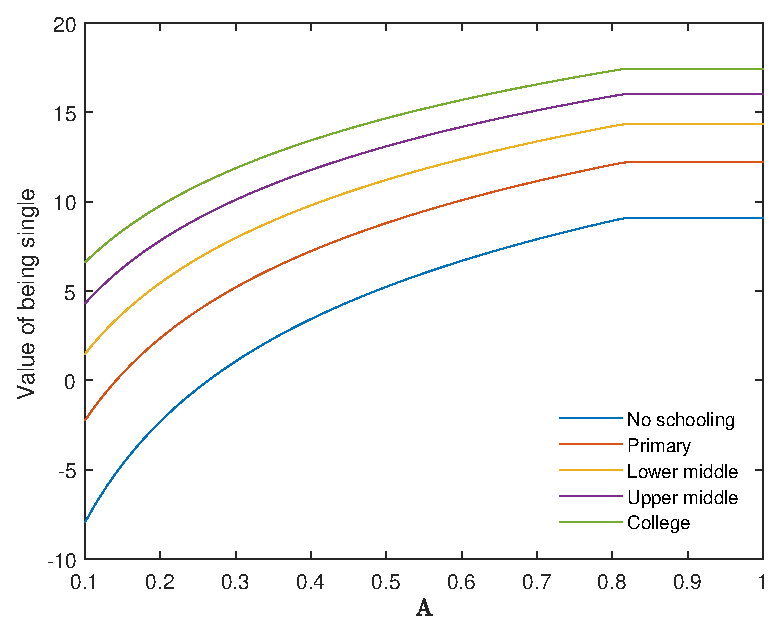
\includegraphics{Graphs/VS_f_A_ex1.eps}} \\
	\subfigure[Males]{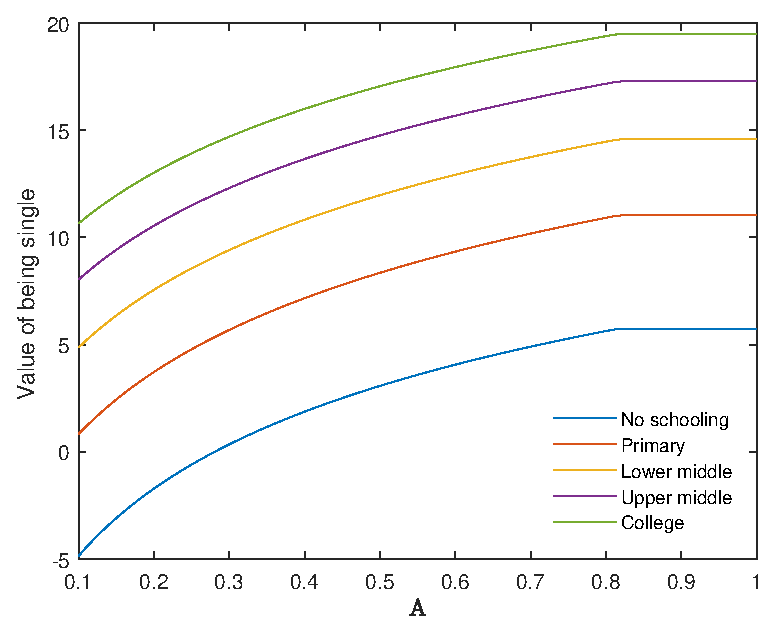
\includegraphics{Graphs/VS_m_A_ex1.eps}}
\end{figure}


\begin{figure}
	\centering
	\caption{Matching probability by sex}
	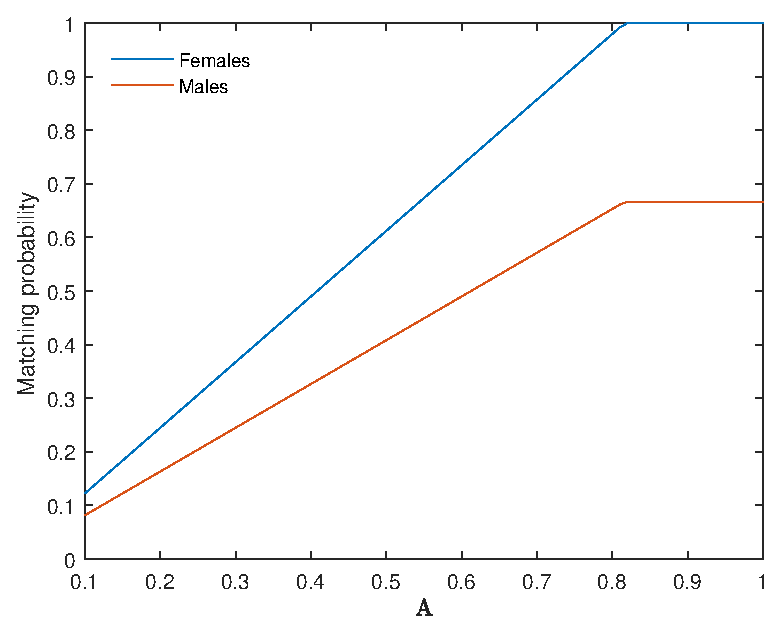
\includegraphics{Graphs/match_prob_A_ex1.eps}
\end{figure}

\begin{figure}
	\centering
	\caption{Marriage rates by sex}
	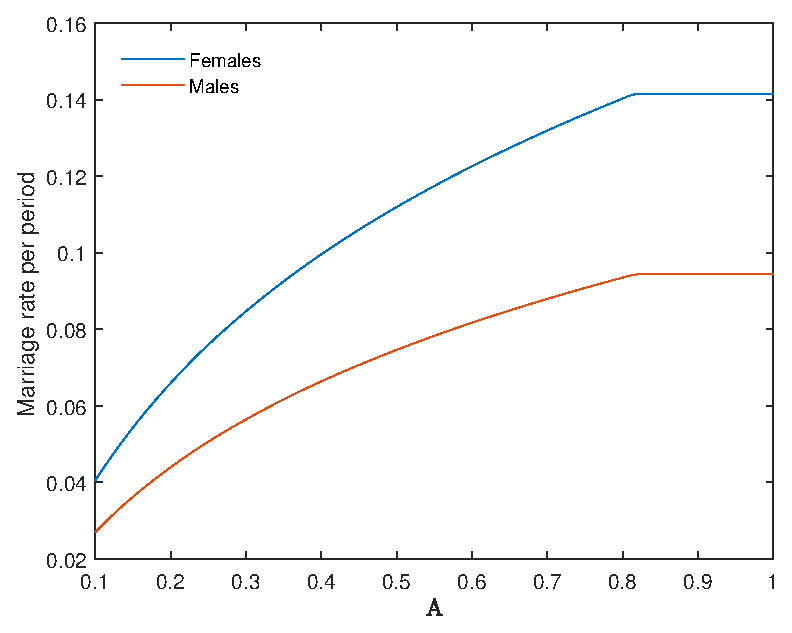
\includegraphics{Graphs/marr_rates_A_ex1.eps}
\end{figure}

\begin{figure}
	\centering
	\caption{Marriage rates by education level}
	\subfigure[Females]{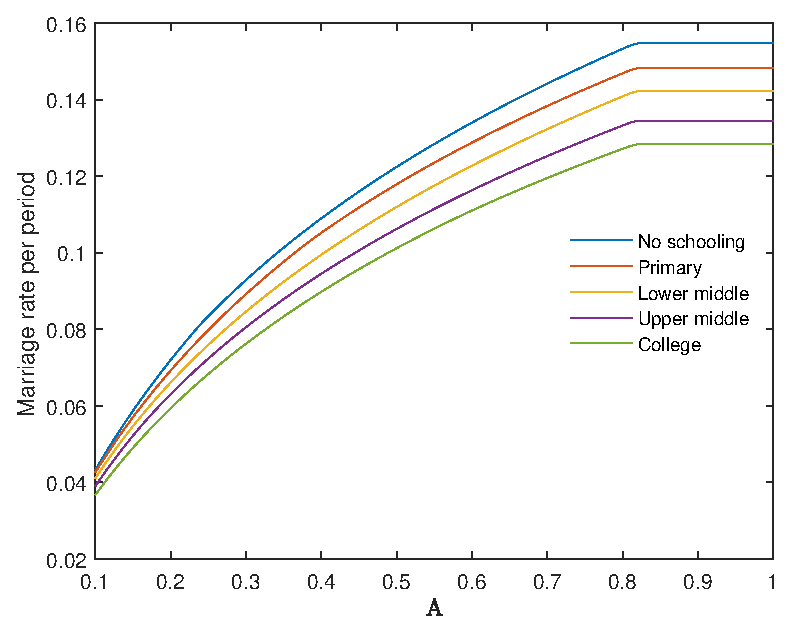
\includegraphics{Graphs/MR_f_A_ex1.eps}} \\
	\subfigure[Males]{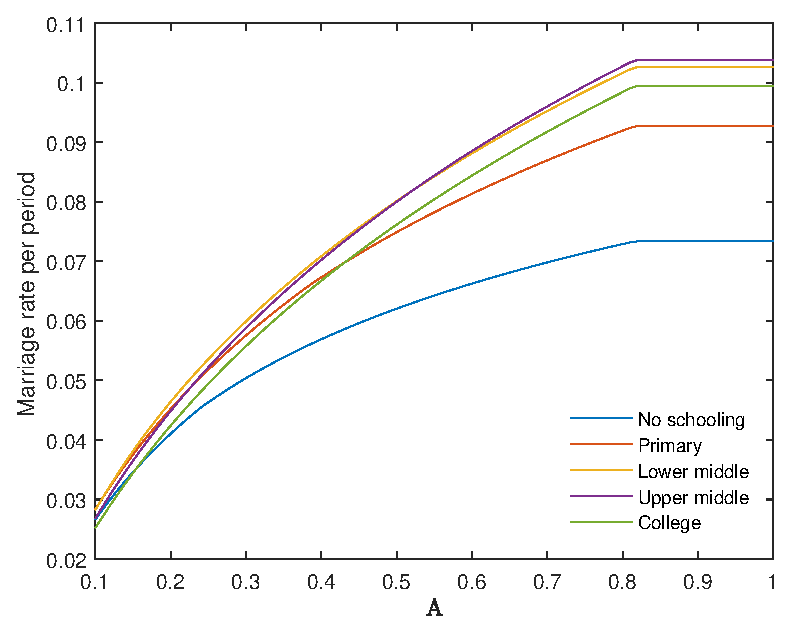
\includegraphics{Graphs/MR_m_A_ex1.eps}}
\end{figure}

\begin{figure}
	\centering
	\caption{Marital sorting in education}
	\subfigure[Basis: only married people]{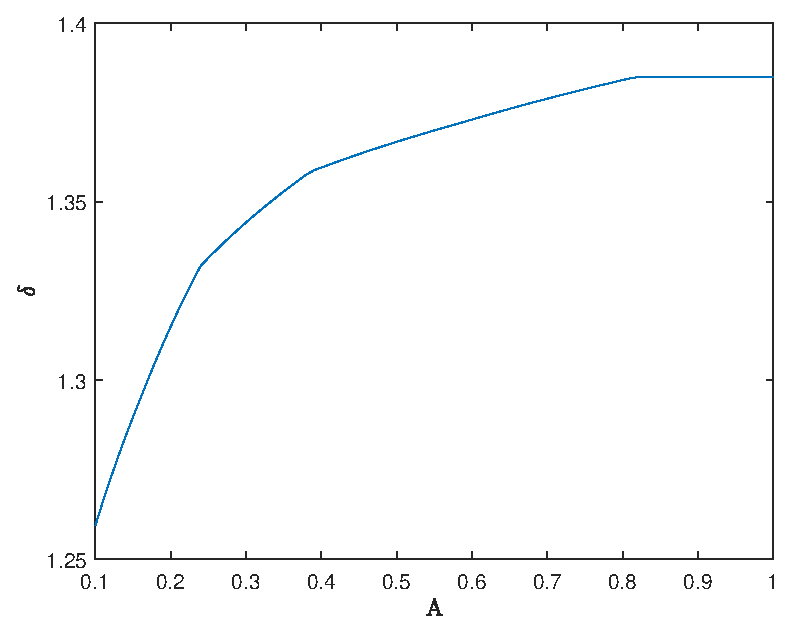
\includegraphics{Graphs/sorting_A_ex1.eps}} \\
	\subfigure[Basis: all individuals]{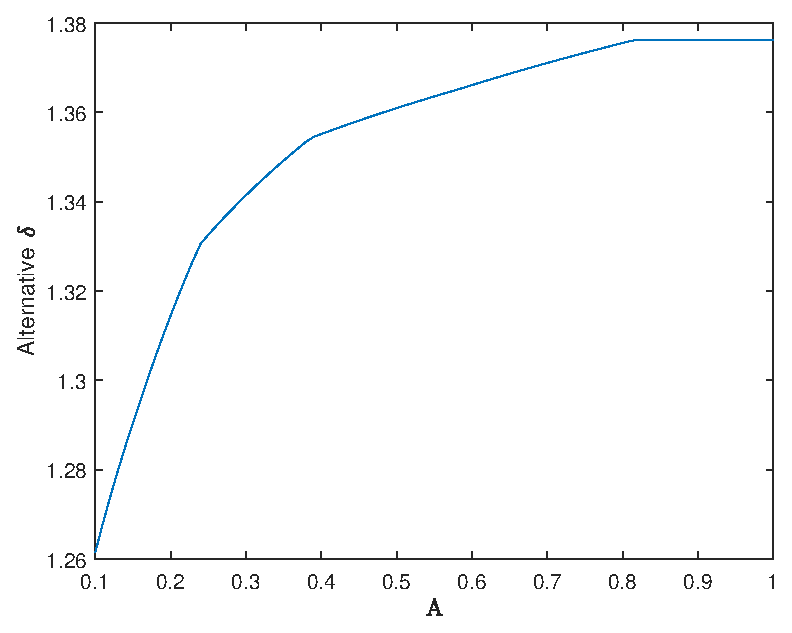
\includegraphics{Graphs/sorting_2_A_ex1.eps}}
\end{figure}

\begin{figure}
	\centering
	\caption{Hypergamy in education by sex}
	\subfigure[Basis: only married people]{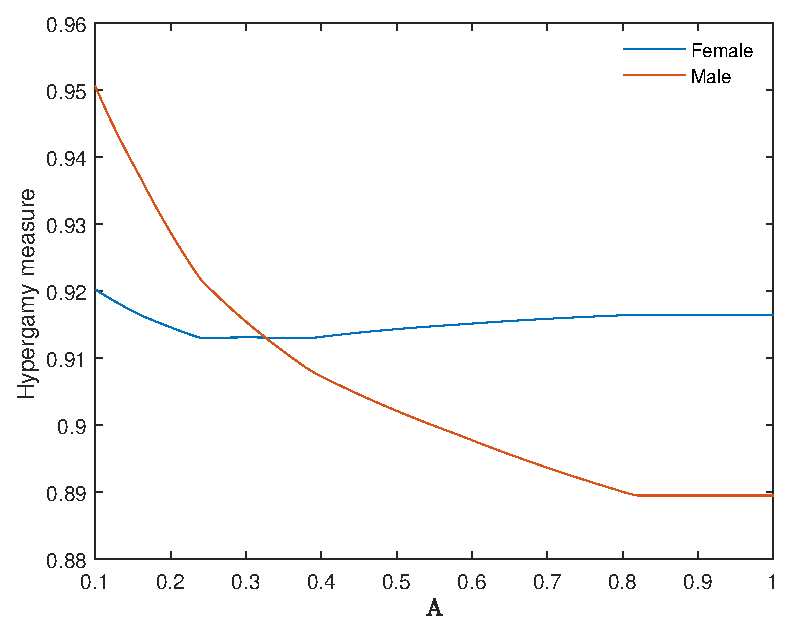
\includegraphics{Graphs/hypergamy_A_ex1.eps}} \\
	\subfigure[Basis: all individuals]{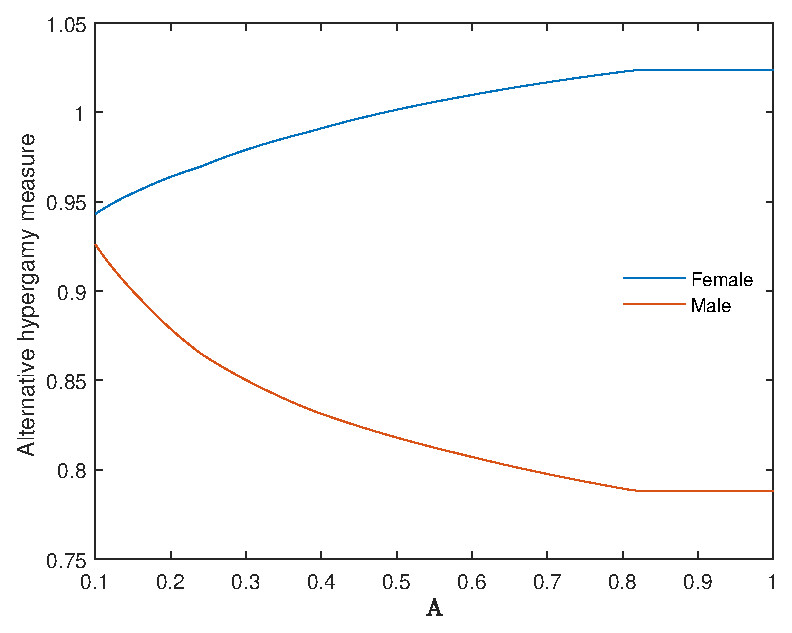
\includegraphics{Graphs/hypergamy_2_A_ex1.eps}}
\end{figure}


\begin{figure}
	\centering
	\caption{Expected time to marriage}
	\includegraphics{Graphs/exp_single_A_ex1.eps}
\end{figure}

\begin{figure}
	\centering
	\caption{Married female labor supply}
	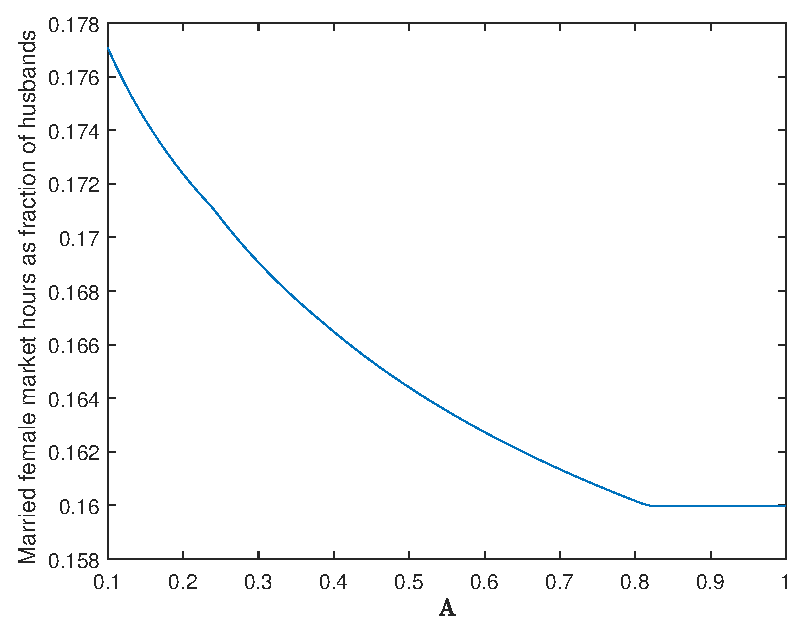
\includegraphics{Graphs/lf_A_ex1.eps}
\end{figure}

\begin{figure}
	\centering
	\caption{Inequality}
	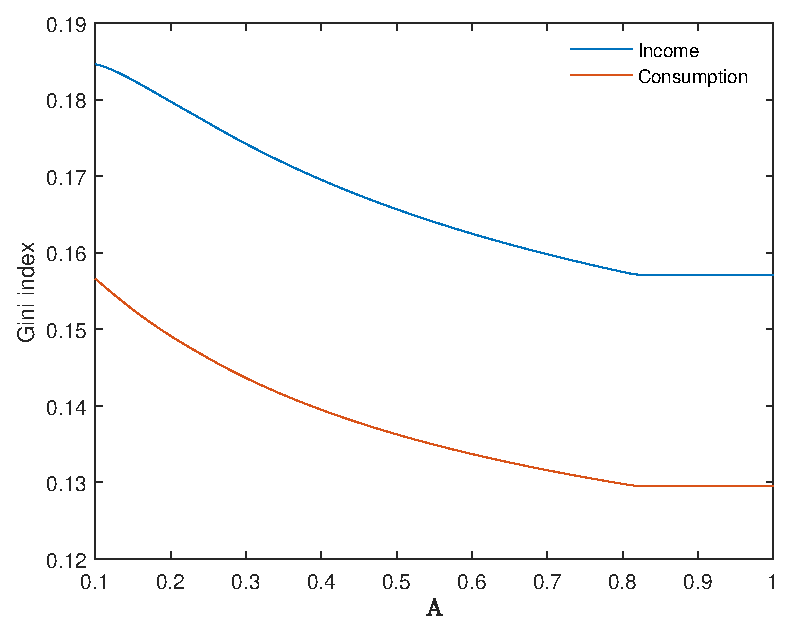
\includegraphics{Graphs/ineq_A_ex1.eps}
\end{figure}

Notes:

\begin{enumerate}
	\item 
\end{enumerate}

\clearpage

\section{Comparative statics on $\kappa$}

\subsection{Exercise 1}

\begin{table}[htbp]
	\centering
	\caption{Parameters for exercise 1}
	\begin{tabular}{lr}
		\toprule
		Parameter & \multicolumn{1}{l}{Value} \\
		\midrule
		&  \\
		Periods per year & 1,000 \\
		$\beta$ & 0,960 \\
		Life expectancy & 45,000 \\
		$\delta$ & 0,022 \\
		$A$ & 0,500 \\
		$\alpha$ & 0,500 \\
		$\bar {c}$ & 0,500 \\
		$\lambda$ & 0,500 \\
		$\gamma$ & 1,500 \\
		&  \\
		$\theta_S$ & 1,500 \\
		&  \\
		Gender wage gap & 0,750 \\
		Skill premium & 0,250 \\
		General wage level & 1,000 \\
		\bottomrule
	\end{tabular}
\end{table}

\begin{figure}
	\centering
	\caption{Value of being single}
	\subfigure[Females]{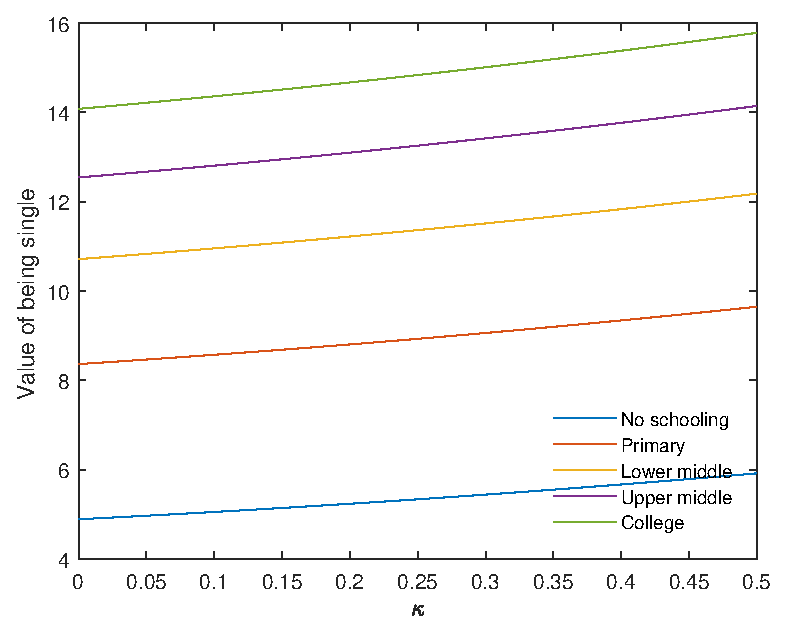
\includegraphics{Graphs/VS_f_kappa_ex1.eps}} \\
	\subfigure[Males]{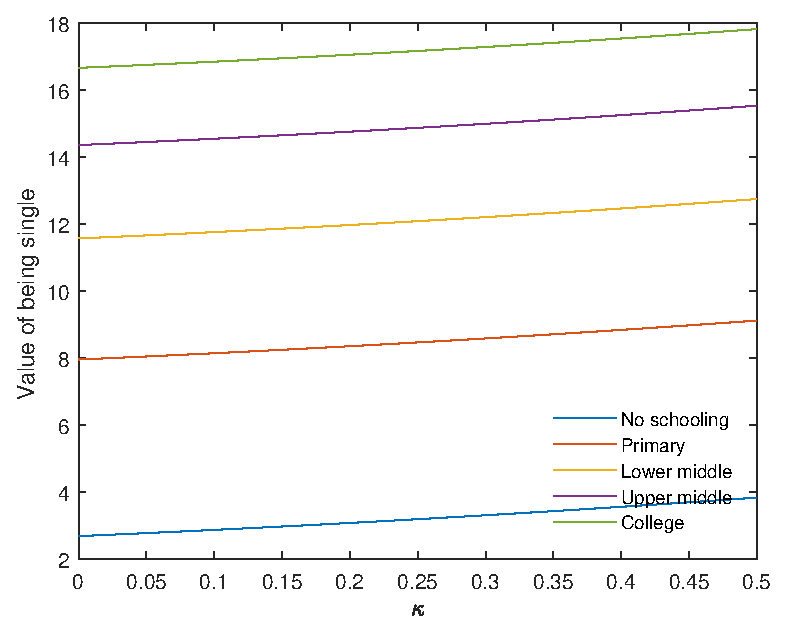
\includegraphics{Graphs/VS_m_kappa_ex1.eps}}
\end{figure}


\begin{figure}
	\centering
	\caption{Matching probability by sex}
	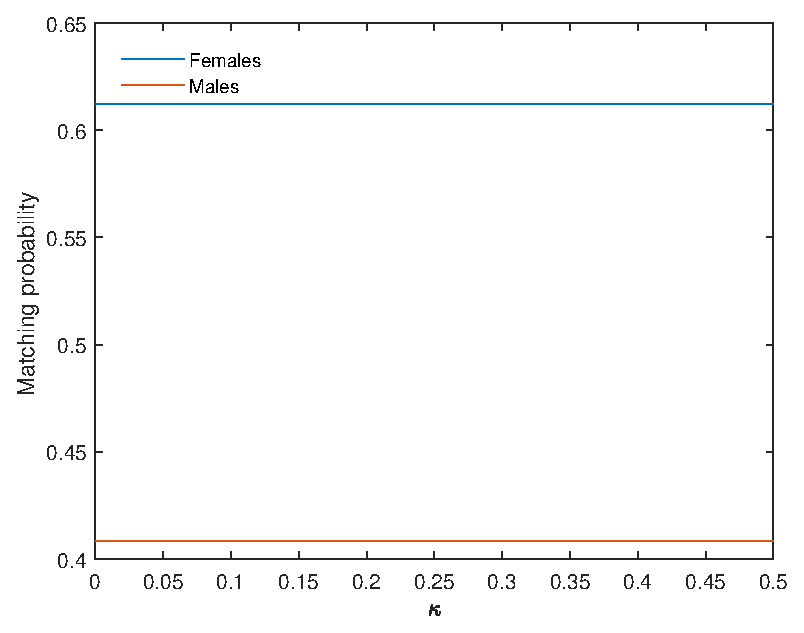
\includegraphics{Graphs/match_prob_kappa_ex1.eps}
\end{figure}

\begin{figure}
	\centering
	\caption{Marriage rates by sex}
	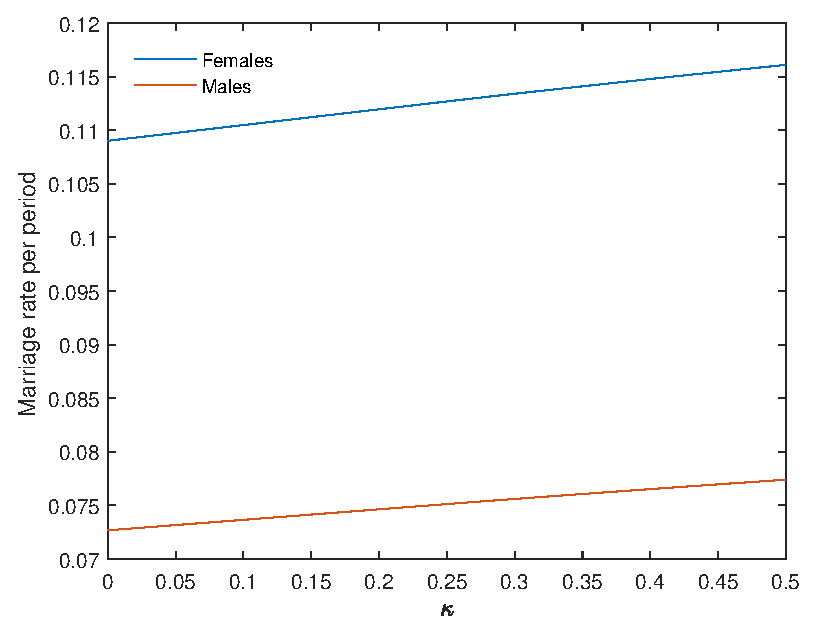
\includegraphics{Graphs/marr_rates_kappa_ex1.eps}
\end{figure}

\begin{figure}
	\centering
	\caption{Marriage rates by education level}
	\subfigure[Females]{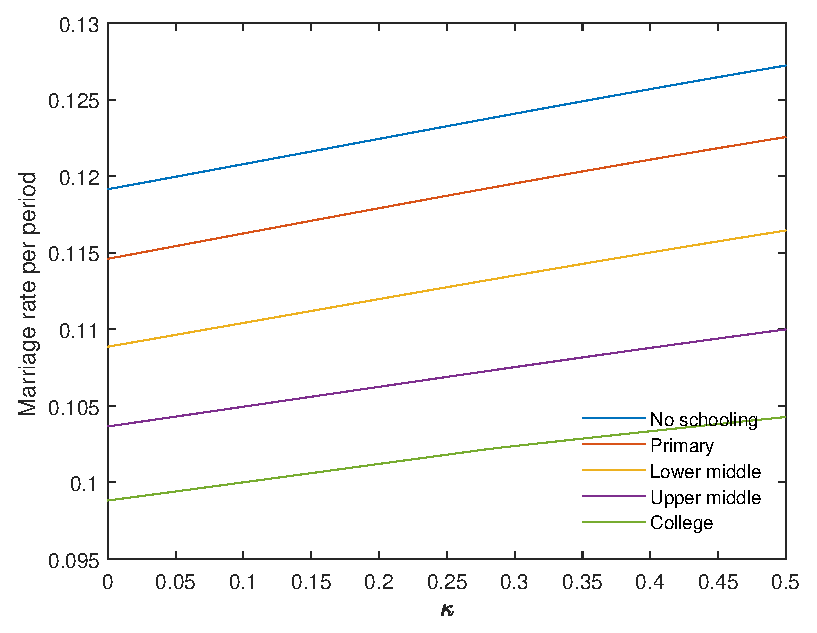
\includegraphics{Graphs/MR_f_kappa_ex1.eps}} \\
	\subfigure[Males]{\includegraphics{Graphs/MR_m_kappa_ex1.eps}}
\end{figure}

\begin{figure}
	\centering
	\caption{Marital sorting in education}
	\subfigure[Basis: only married people]{\includegraphics{Graphs/sorting_kappa_ex1.eps}} \\
	\subfigure[Basis: all individuals]{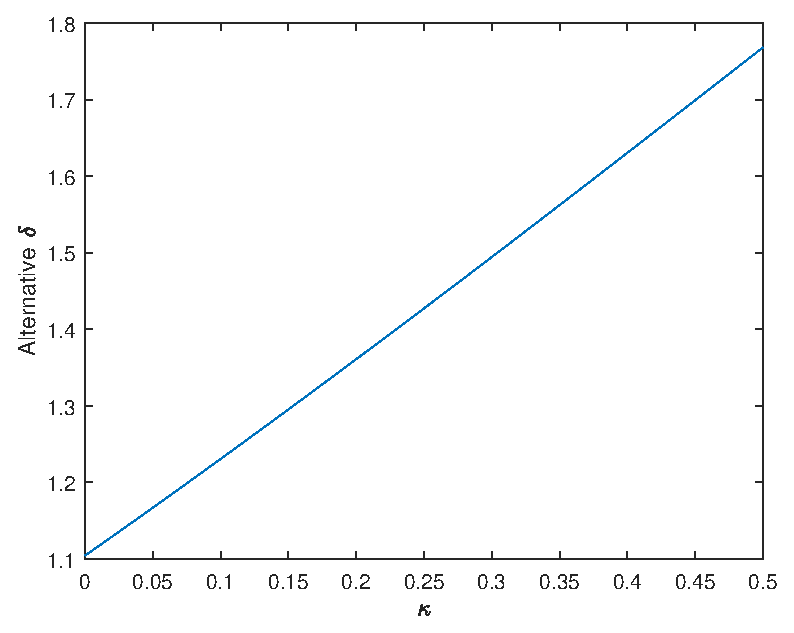
\includegraphics{Graphs/sorting_2_kappa_ex1.eps}}
\end{figure}

\begin{figure}
	\centering
	\caption{Hypergamy in education by sex}
	\subfigure[Basis: only married people]{\includegraphics{Graphs/hypergamy_kappa_ex1.eps}} \\
	\subfigure[Basis: all individuals]{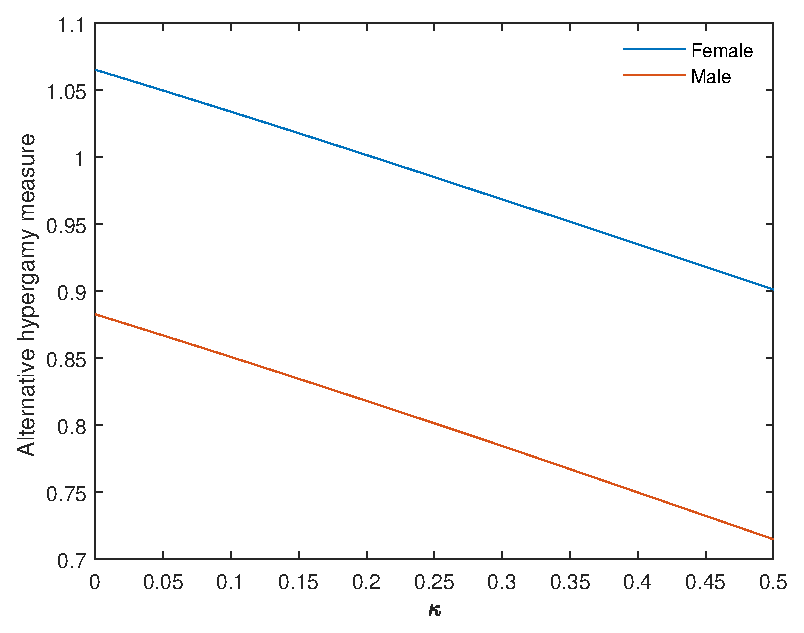
\includegraphics{Graphs/hypergamy_2_kappa_ex1.eps}}
\end{figure}


\begin{figure}
	\centering
	\caption{Expected time to marriage}
	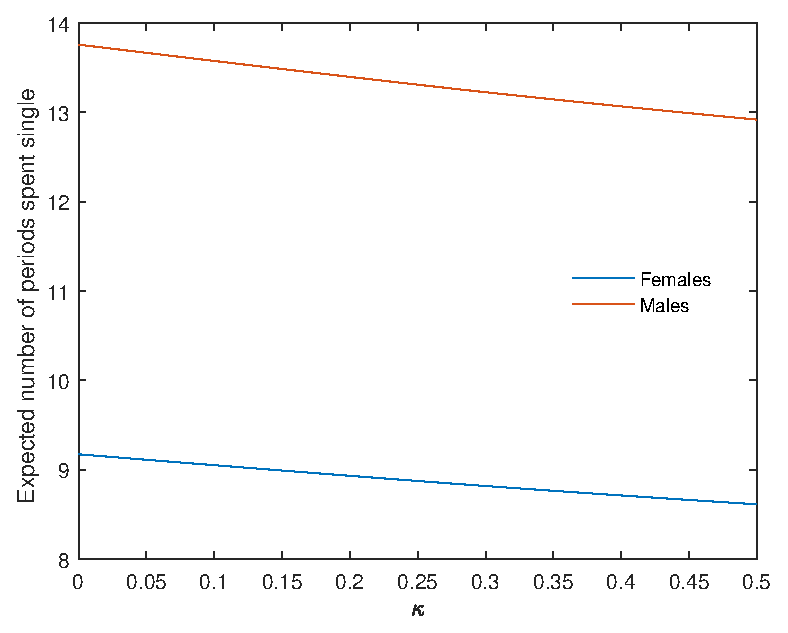
\includegraphics{Graphs/exp_single_kappa_ex1.eps}
\end{figure}

\begin{figure}
	\centering
	\caption{Married female labor supply}
	\includegraphics{Graphs/lf_kappa_ex1.eps}
\end{figure}

\begin{figure}
	\centering
	\caption{Inequality}
	\includegraphics{Graphs/ineq_kappa_ex1.eps}
\end{figure}

Notes:

\begin{enumerate}
	\item 
\end{enumerate}

\clearpage

\section{Comparative statics on $\bar{c}$}

\subsection{Exercise 1}

\begin{table}[htbp]
	\centering
	\caption{Parameters for exercise 1}
	\begin{tabular}{lr}
		\toprule
		Parameter & \multicolumn{1}{l}{Value} \\
		\midrule
		&  \\
		Periods per year & 1,000 \\
		$\beta$ & 0,960 \\
		Life expectancy & 45,000 \\
		$\delta$ & 0,022 \\
		$A$ & 0,500 \\
		$\alpha$ & 0,500 \\
		$\kappa$ & 0,200 \\
		$\lambda$ & 0,500 \\
		$\gamma$ & 1,500 \\
		&  \\
		$\theta_S$ & 1,500 \\
		&  \\
		Gender wage gap & 0,750 \\
		Skill premium & 0,250 \\
		General wage level & 1,000 \\
		\bottomrule
	\end{tabular}
\end{table}

\begin{figure}
	\centering
	\caption{Value of being single}
	\subfigure[Females]{\includegraphics{Graphs/VS_f_cbar_ex1.eps}} \\
	\subfigure[Males]{\includegraphics{Graphs/VS_m_cbar_ex1.eps}}
\end{figure}


\begin{figure}
	\centering
	\caption{Matching probability by sex}
	\includegraphics{Graphs/match_prob_cbar_ex1.eps}
\end{figure}

\begin{figure}
	\centering
	\caption{Marriage rates by sex}
	\includegraphics{Graphs/marr_rates_cbar_ex1.eps}
\end{figure}

\begin{figure}
	\centering
	\caption{Marriage rates by education level}
	\subfigure[Females]{\includegraphics{Graphs/MR_f_cbar_ex1.eps}} \\
	\subfigure[Males]{\includegraphics{Graphs/MR_m_cbar_ex1.eps}}
\end{figure}

\begin{figure}
	\centering
	\caption{Marital sorting in education}
	\subfigure[Basis: only married people]{\includegraphics{Graphs/sorting_cbar_ex1.eps}} \\
	\subfigure[Basis: all individuals]{\includegraphics{Graphs/sorting_2_cbar_ex1.eps}}
\end{figure}

\begin{figure}
	\centering
	\caption{Hypergamy in education by sex}
	\subfigure[Basis: only married people]{\includegraphics{Graphs/hypergamy_cbar_ex1.eps}} \\
	\subfigure[Basis: all individuals]{\includegraphics{Graphs/hypergamy_2_cbar_ex1.eps}}
\end{figure}


\begin{figure}
	\centering
	\caption{Expected time to marriage}
	\includegraphics{Graphs/exp_single_cbar_ex1.eps}
\end{figure}

\begin{figure}
	\centering
	\caption{Married female labor supply}
	\includegraphics{Graphs/lf_cbar_ex1.eps}
\end{figure}

\begin{figure}
	\centering
	\caption{Inequality}
	\includegraphics{Graphs/ineq_cbar_ex1.eps}
\end{figure}

Notes:

\begin{enumerate}
	\item 
\end{enumerate}

\clearpage

\section{Comparative statics on $\lambda$}

\subsection{Exercise 1}

\begin{table}[htbp]
	\centering
	\caption{Parameters for exercise 1}
	\begin{tabular}{lr}
		\toprule
		Parameter & \multicolumn{1}{l}{Value} \\
		\midrule
		&  \\
		Periods per year & 1,000 \\
		$\beta$ & 0,960 \\
		Life expectancy & 45,000 \\
		$\delta$ & 0,022 \\
		$A$ & 0,500 \\
		$\alpha$ & 0,500 \\
		$\kappa$ & 0,200 \\
		$\bar {c}$ & 0,500 \\
		$\gamma$ & 1,500 \\
		&  \\
		$\theta_S$ & 1,500 \\
		&  \\
		Gender wage gap & 0,750 \\
		Skill premium & 0,250 \\
		General wage level & 1,000 \\
		\bottomrule
	\end{tabular}
\end{table}

\begin{figure}
	\centering
	\caption{Value of being single}
	\subfigure[Females]{\includegraphics{Graphs/VS_f_lambda_ex1.eps}} \\
	\subfigure[Males]{\includegraphics{Graphs/VS_m_lambda_ex1.eps}}
\end{figure}


\begin{figure}
	\centering
	\caption{Matching probability by sex}
	\includegraphics{Graphs/match_prob_lambda_ex1.eps}
\end{figure}

\begin{figure}
	\centering
	\caption{Marriage rates by sex}
	\includegraphics{Graphs/marr_rates_lambda_ex1.eps}
\end{figure}

\begin{figure}
	\centering
	\caption{Marriage rates by education level}
	\subfigure[Females]{\includegraphics{Graphs/MR_f_lambda_ex1.eps}} \\
	\subfigure[Males]{\includegraphics{Graphs/MR_m_lambda_ex1.eps}}
\end{figure}

\begin{figure}
	\centering
	\caption{Marital sorting in education}
	\subfigure[Basis: only married people]{\includegraphics{Graphs/sorting_lambda_ex1.eps}} \\
	\subfigure[Basis: all individuals]{\includegraphics{Graphs/sorting_2_lambda_ex1.eps}}
\end{figure}

\begin{figure}
	\centering
	\caption{Hypergamy in education by sex}
	\subfigure[Basis: only married people]{\includegraphics{Graphs/hypergamy_lambda_ex1.eps}} \\
	\subfigure[Basis: all individuals]{\includegraphics{Graphs/hypergamy_2_lambda_ex1.eps}}
\end{figure}


\begin{figure}
	\centering
	\caption{Expected time to marriage}
	\includegraphics{Graphs/exp_single_lambda_ex1.eps}
\end{figure}

\begin{figure}
	\centering
	\caption{Married female labor supply}
	\includegraphics{Graphs/lf_lambda_ex1.eps}
\end{figure}

\begin{figure}
	\centering
	\caption{Inequality}
	\includegraphics{Graphs/ineq_lambda_ex1.eps}
\end{figure}

Notes:

\begin{enumerate}
	\item 
\end{enumerate}

\clearpage

\section{Comparative statics on $\gamma$}

\subsection{Exercise 1}

\begin{table}[htbp]
	\centering
	\caption{Parameters for exercise 1}
	\begin{tabular}{lr}
		\toprule
		Parameter & \multicolumn{1}{l}{Value} \\
		\midrule
		&  \\
		Periods per year & 1,000 \\
		$\beta$ & 0,960 \\
		Life expectancy & 45,000 \\
		$\delta$ & 0,022 \\
		$A$ & 0,500 \\
		$\alpha$ & 0,500 \\
		$\kappa$ & 0,200 \\
		$\bar {c}$ & 0,500 \\
		$\lambda$ & 0,500 \\
		&  \\
		$\theta_S$ & 1,500 \\
		&  \\
		Gender wage gap & 0,750 \\
		Skill premium & 0,250 \\
		General wage level & 1,000 \\
		\bottomrule
	\end{tabular}
\end{table}

\begin{figure}
	\centering
	\caption{Value of being single}
	\subfigure[Females]{\includegraphics{Graphs/VS_f_gamma_ex1.eps}} \\
	\subfigure[Males]{\includegraphics{Graphs/VS_m_gamma_ex1.eps}}
\end{figure}


\begin{figure}
	\centering
	\caption{Matching probability by sex}
	\includegraphics{Graphs/match_prob_gamma_ex1.eps}
\end{figure}

\begin{figure}
	\centering
	\caption{Marriage rates by sex}
	\includegraphics{Graphs/marr_rates_gamma_ex1.eps}
\end{figure}

\begin{figure}
	\centering
	\caption{Marriage rates by education level}
	\subfigure[Females]{\includegraphics{Graphs/MR_f_gamma_ex1.eps}} \\
	\subfigure[Males]{\includegraphics{Graphs/MR_m_gamma_ex1.eps}}
\end{figure}

\begin{figure}
	\centering
	\caption{Marital sorting in education}
	\subfigure[Basis: only married people]{\includegraphics{Graphs/sorting_gamma_ex1.eps}} \\
	\subfigure[Basis: all individuals]{\includegraphics{Graphs/sorting_2_gamma_ex1.eps}}
\end{figure}

\begin{figure}
	\centering
	\caption{Hypergamy in education by sex}
	\subfigure[Basis: only married people]{\includegraphics{Graphs/hypergamy_gamma_ex1.eps}} \\
	\subfigure[Basis: all individuals]{\includegraphics{Graphs/hypergamy_2_gamma_ex1.eps}}
\end{figure}


\begin{figure}
	\centering
	\caption{Expected time to marriage}
	\includegraphics{Graphs/exp_single_gamma_ex1.eps}
\end{figure}

\begin{figure}
	\centering
	\caption{Married female labor supply}
	\includegraphics{Graphs/lf_gamma_ex1.eps}
\end{figure}

\begin{figure}
	\centering
	\caption{Inequality}
	\includegraphics{Graphs/ineq_gamma_ex1.eps}
\end{figure}

Notes:

\begin{enumerate}
	\item 
\end{enumerate}

\clearpage

\section{Comparative statics on the general wage level}

\subsection{Exercise 1}

\begin{table}[htbp]
	\centering
	\caption{Parameters for exercise 1}
	\begin{tabular}{lr}
		\toprule
		Parameter & \multicolumn{1}{l}{Value} \\
		\midrule
		&  \\
		Periods per year & 1,000 \\
		$\beta$ & 0,960 \\
		Life expectancy & 45,000 \\
		$\delta$ & 0,022 \\
		$A$ & 0,500 \\
		$\alpha$ & 0,500 \\
		$\kappa$ & 0,200 \\
		$\bar {c}$ & 0,500 \\
		$\lambda$ & 0,500 \\
		$\gamma$ & 1,500 \\
		&  \\
		$\theta_S$ & 1,500 \\
		&  \\
		Gender wage gap & 0,750 \\
		Skill premium & 0,250 \\
		General wage level & 1,000 \\
		\bottomrule
	\end{tabular}%
\end{table}

\begin{figure}
	\centering
	\caption{Value of being single}
	\subfigure[Females]{\includegraphics{Graphs/VS_f_general_wage_ex1.eps}} \\
	\subfigure[Males]{\includegraphics{Graphs/VS_m_general_wage_ex1.eps}}
\end{figure}


\begin{figure}
	\centering
	\caption{Matching probability by sex}
	\includegraphics{Graphs/match_prob_general_wage_ex1.eps}
\end{figure}

\begin{figure}
	\centering
	\caption{Marriage rates by sex}
	\includegraphics{Graphs/marr_rates_general_wage_ex1.eps}
\end{figure}

\begin{figure}
	\centering
	\caption{Marriage rates by education level}
	\subfigure[Females]{\includegraphics{Graphs/MR_f_general_wage_ex1.eps}} \\
	\subfigure[Males]{\includegraphics{Graphs/MR_m_general_wage_ex1.eps}}
\end{figure}

\begin{figure}
	\centering
	\caption{Marital sorting in education}
	\subfigure[Basis: only married people]{\includegraphics{Graphs/sorting_general_wage_ex1.eps}} \\
	\subfigure[Basis: all individuals]{\includegraphics{Graphs/sorting_2_general_wage_ex1.eps}}
\end{figure}

\begin{figure}
	\centering
	\caption{Hypergamy in education by sex}
	\subfigure[Basis: only married people]{\includegraphics{Graphs/hypergamy_general_wage_ex1.eps}} \\
	\subfigure[Basis: all individuals]{\includegraphics{Graphs/hypergamy_2_general_wage_ex1.eps}}
\end{figure}


\begin{figure}
	\centering
	\caption{Expected time to marriage}
	\includegraphics{Graphs/exp_single_general_wage_ex1.eps}
\end{figure}

\begin{figure}
	\centering
	\caption{Married female labor supply}
	\includegraphics{Graphs/lf_general_wage_ex1.eps}
\end{figure}

\begin{figure}
	\centering
	\caption{Inequality}
	\includegraphics{Graphs/ineq_general_wage_ex1.eps}
\end{figure}

Notes:

\begin{enumerate}
	\item 
\end{enumerate}

\clearpage

\end{document}